	The previous version of the MVSS sensor could only attain a maximum synchronized frame rate of 0.5Hz, which is inadequate for celerity based bathymetry inversions.  Alternative sensors were assessed and considered, with cost and weight being the major limitations.  After consideration, an array of GoPro Hero 4 Black sensors with modified lenses were selected as the camera sensors. 
	\section{Camera Selection}
	\subsection{GoPro Hero 4 Black}
	GoPro cameras are a Commercial Off The Shelf(COTS) camera that is used by consumers across the world for video and imagery.  While the GoPro sensors have a number of negatives, outlined in the advantages and disadvantages list in \tabref{tab:gopro}, they were ultimately selected due to the low weight, low cost, low power, availability for purchase, and ruggedness of the cameras.
	
	\begin{table}[H]
		\begin{tabularx}{\linewidth}{>{\parskip1ex}X@{\kern4\tabcolsep}>{\parskip1ex}X}
			\toprule
			\hfil\bfseries Advantages
			&
			\hfil\bfseries Disadvantages
			\\\cmidrule(r{3\tabcolsep}){1-1}\cmidrule(l{-\tabcolsep}){2-2}
			Inexpensive\par
			Lightweight\par
			Easy to purchase\par
			Rugged\par
			Low Power Requirements
			&
			CMOS rolling shutter (nonlinear image distortion)\par
			No documented method for time synchronization\par
			High lens distortion 
			\\\bottomrule
		\end{tabularx}
		\caption{Advantages and disadvantages of using GoPro cameras for use in the second version of the MVSS.}
		\label{tab:gopro}
	\end{table}
	
	\subsection{PtGrey}
	PtGrey is an industrial camera manufacturer that manufacturers a wide array of products which contain hardware triggering.  While the hardware triggering of these sensors would be a much more robust and accurate time synchronization methodology, the weight and power requirements were too great for integration on a small Unmanned Aerial System.  The PtGrey Ladybug was also considered, but the weight and power for it made integration on a UAS prohibitive. An advantages and disadvantages list for the PtGrey cameras is shown in \tabref{tab:PtGrey}.
	
	\begin{table}[H]
		\begin{tabularx}{\linewidth}{>{\parskip1ex}X@{\kern4\tabcolsep}>{\parskip1ex}X}
			\toprule
			\hfil\bfseries Advantages
			&
			\hfil\bfseries Disadvantages
			\\\cmidrule(r{3\tabcolsep}){1-1}\cmidrule(l{-\tabcolsep}){2-2}
			Hardware triggering\par
			Well documented API\par
			Reliable\par
			Many Lens Options\par
			&
			Too heavy with lenses and CPU\par
			Requires external CPU for triggering and data storage\par
			Requires a lot of power to run the camera and CPU
			\\\bottomrule
		\end{tabularx}
		\caption{Advantages and disadvantages of using PtGrey cameras for use in the second version of the MVSS.}
		\label{tab:PtGrey}
	\end{table}
	
	\subsection{Raspberry Pi Camera Module}
	Raspberry Pi is an inexpensive, consumer grade linux computer that is marketed towards students and hobbyists.  The Raspberry Pi computer interfaces with a small Raspberry Pi camera module, which can then be used to acquire imagery and video.  After experimenting with the camera, it was determined that the software triggering accuracy of the camera was inadequate for time synchronization across an array of cameras.  The other advantages and disadvantages are shown in \tabref{tab:raspi}.
	
	\begin{table}[H]
		\begin{tabularx}{\linewidth}{>{\parskip1ex}X@{\kern4\tabcolsep}>{\parskip1ex}X}
			\toprule
			\hfil\bfseries Advantages
			&
			\hfil\bfseries Disadvantages
			\\\cmidrule(r{3\tabcolsep}){1-1}\cmidrule(l{-\tabcolsep}){2-2}
			Inexpensive\par
			Lightweight\par
			&
			Low resolution\par
			Inaccurate software trigger\par
			Relatively ``black box'' camera module\par
			Requires a Raspberry Pi for each camera, adding to the power requirements and weight.
			\\\bottomrule
		\end{tabularx}
		\caption{Advantages and disadvantages of using Raspberry Pi cameras for use in the second version of the MVSS.}
		\label{tab:raspi}
	\end{table}
	
	\subsection{CHDK}
	The Canon Hacker Development Kit(CHDK) is an open source project that modifies the firmware of Canon point and shoot cameras to enable advanced image acquisition.  This was used for the first version of MVSS, but the frame rate was too slow.  CHDK was again investigated to see if any improvements could be made to the frame rate, but it was determined that the frame rate could not be improved past the 0.5Hz.
	
	\begin{table}[H]
		\begin{tabularx}{\linewidth}{>{\parskip1ex}X@{\kern4\tabcolsep}>{\parskip1ex}X}
			\toprule
			\hfil\bfseries Advantages
			&
			\hfil\bfseries Disadvantages
			\\\cmidrule(r{3\tabcolsep}){1-1}\cmidrule(l{-\tabcolsep}){2-2}
			Accurate pseudo hardware trigger\par
			High resolution (16Mp)\par
			Lightweight\par
			Low Power\par
			&
			Frequent Undocumented Bugs\par
			Poor Frame Rate\par 
			Retracting Lens causes unstable lens IO parameters
			\\\bottomrule
		\end{tabularx}
		\caption{Advantages and disadvantages of using CHDK cameras for use in the second version of the MVSS.}
		\label{tab:chdk}
	\end{table}
	
	\section{Lens Selection}
	GoPro cameras are constructed with a 2.92mm lens by default, but there is an undocumented method to open the camera and replace the lens. The stock lens mounts into M12 threading, and the whole threading mechanism can be removed and replaced with a product called a ``SuperMount.''  This mount also has M12 threading, but allows for longer focal lengths to be installed.  There were four lenses on the market that advertised a `High Mp' lens for the M12 threading, and each are compared in \figref{fig:lenscomp}.  The 2.9mm after-market lens was eliminated as an option because it exhibited excessive radial distortion and vignetting.  The default, 4.35mm, and 5.4mm lenses were considered as options when designing the camera orientations.   
	
	\begin{figure}[H]
		\centering
		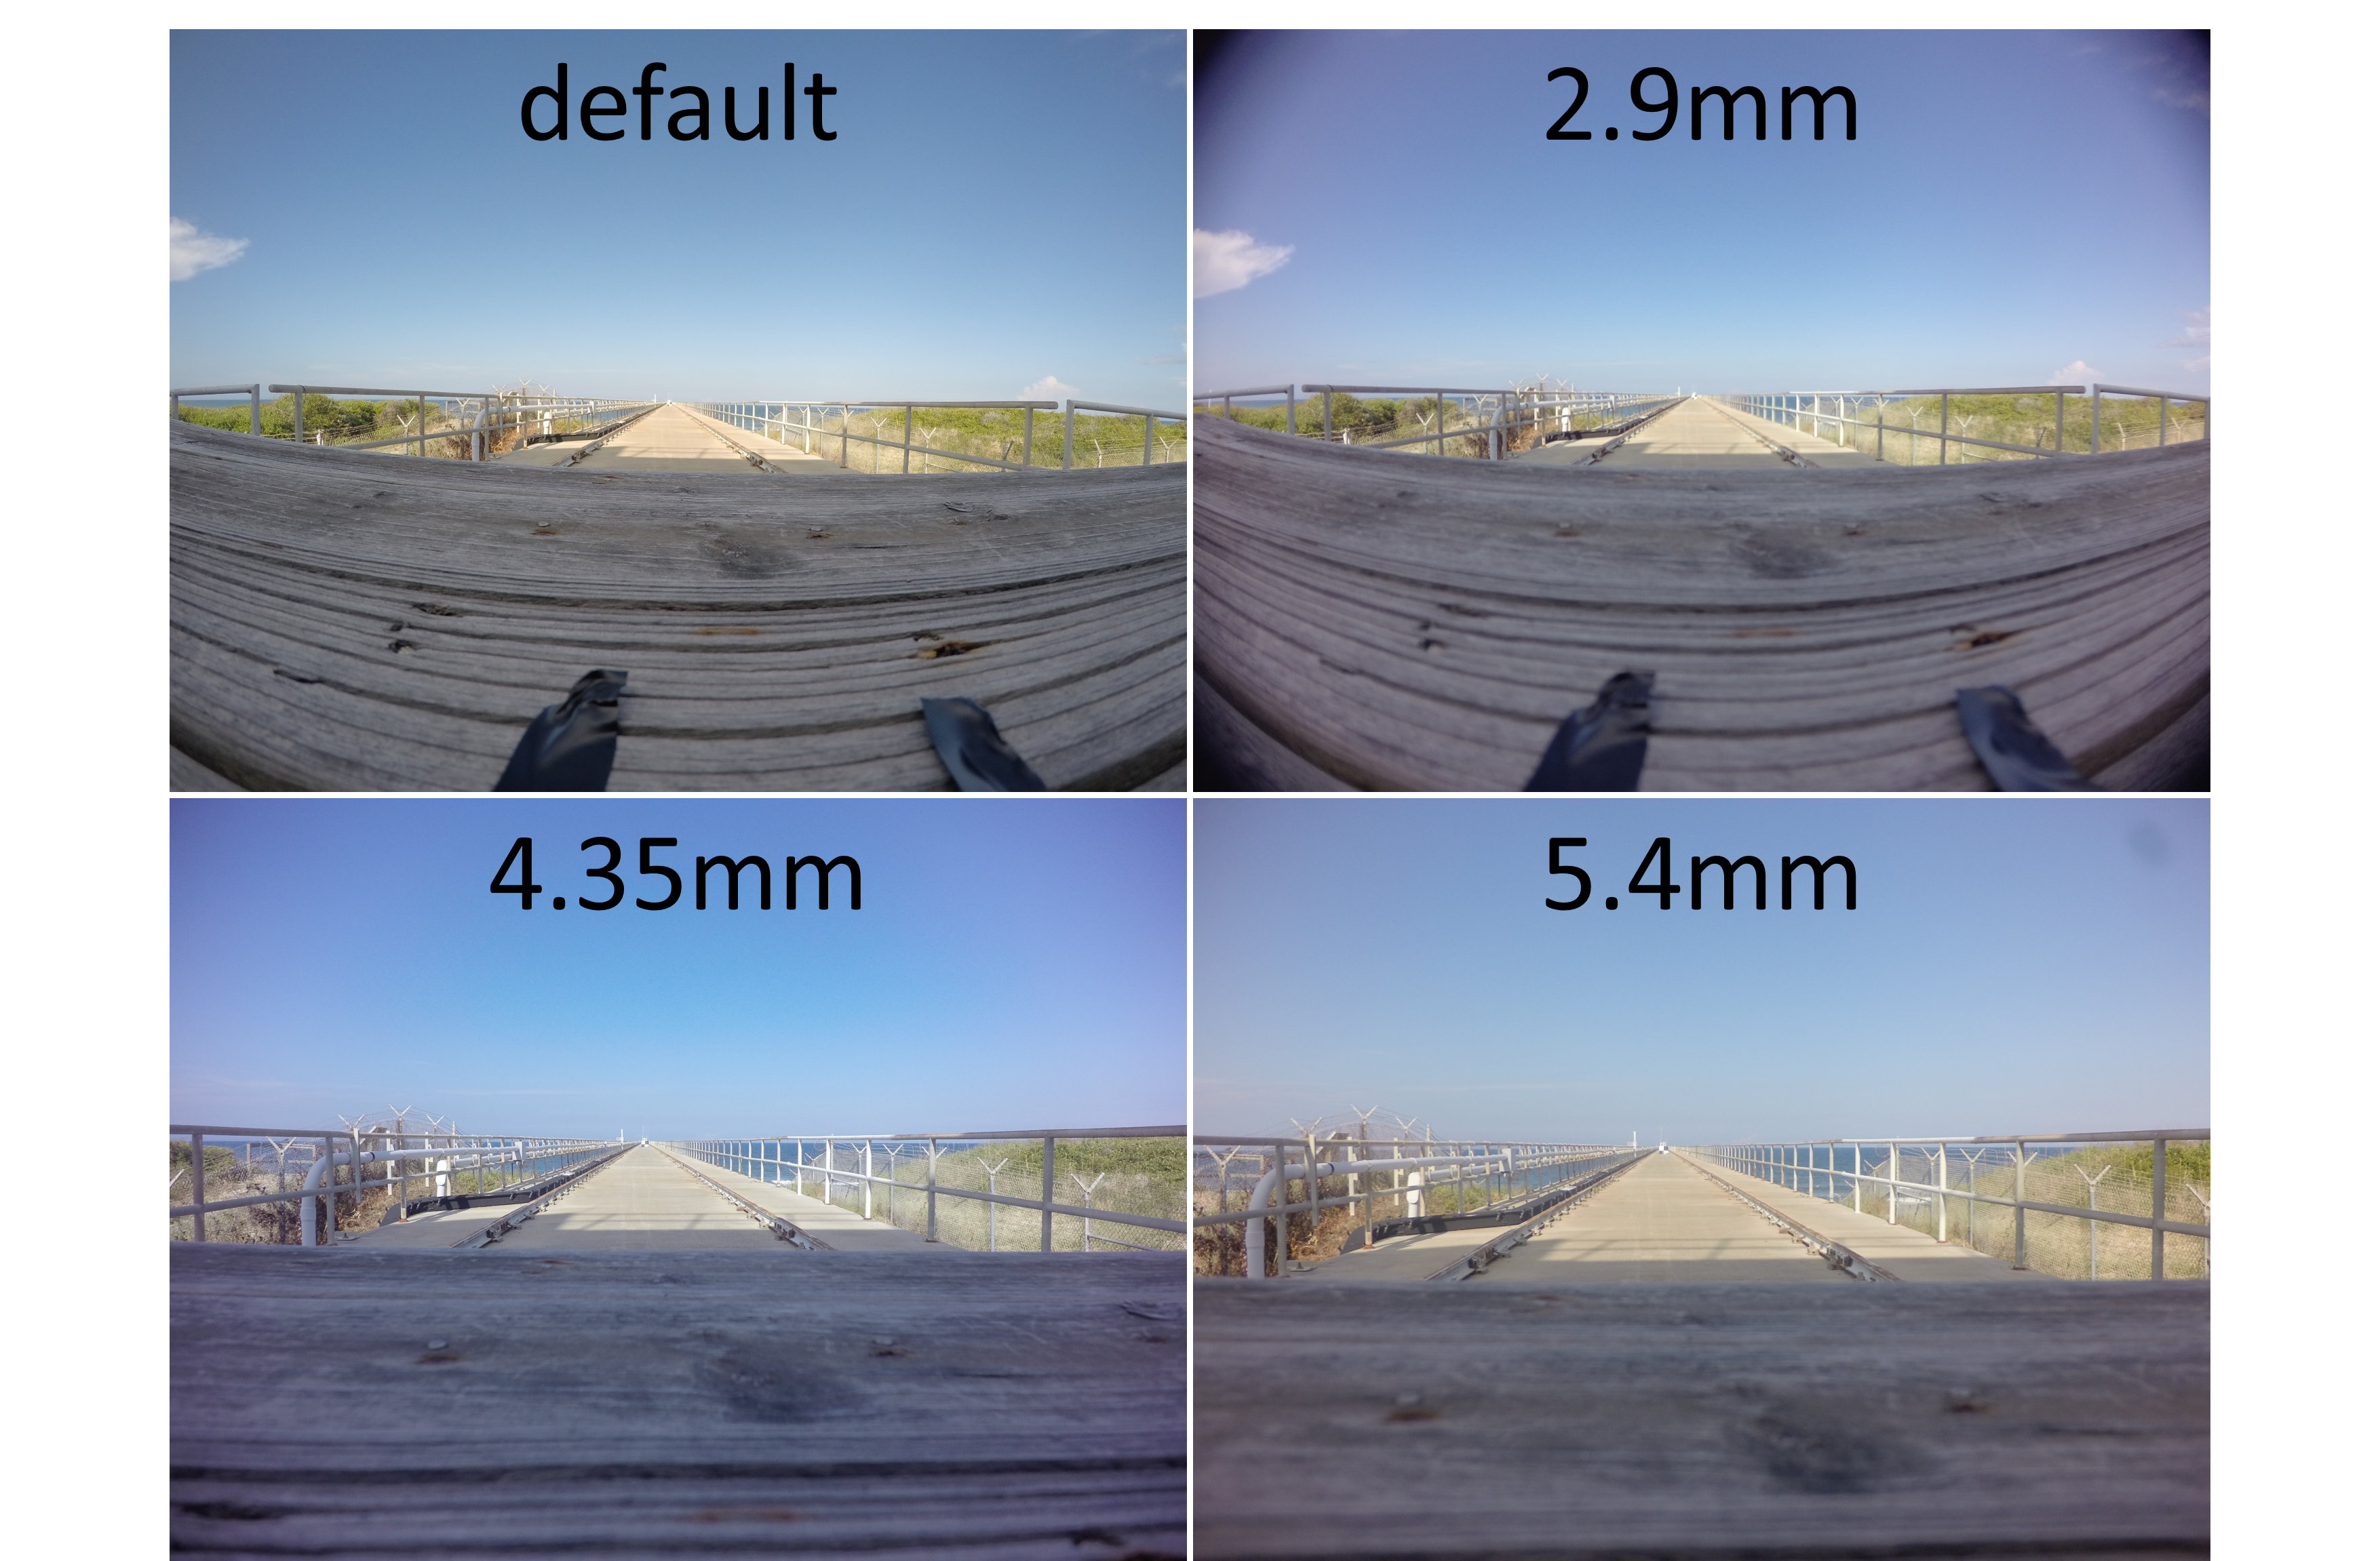
\includegraphics[scale = 0.3]{../figures/lenscomp.png}
		\caption{The four M12 lenses were tested in the GoPro camera, and it was determined that the 2.9mm lens should not be used due to excessive vignetting and distortion.  The default, 4.35mm, and 5.4mm lenses were considered as options when designing the camera orientations.}
		\label{fig:lenscomp}
	\end{figure}

	\section{Possible Improvements}
	The current GoPro sensor design functions as a prototype, but will likely require debugging and troubleshooting to become a robust sensor for repeated data acquisitions.  The GoPro camera is the greatest limiting factor in the system, and efforts should be made to continue explore more robust, industrial camera options as camera technology progresses.  Future work should continue to monitor the virtual reality camera and cell phone camera markets, as these consumer technologies hold great promise for an improved sensor.  These types of cameras may have time synchronization built in, which is the largest issue with this current system.